
\begin{figure*}
	\centering
	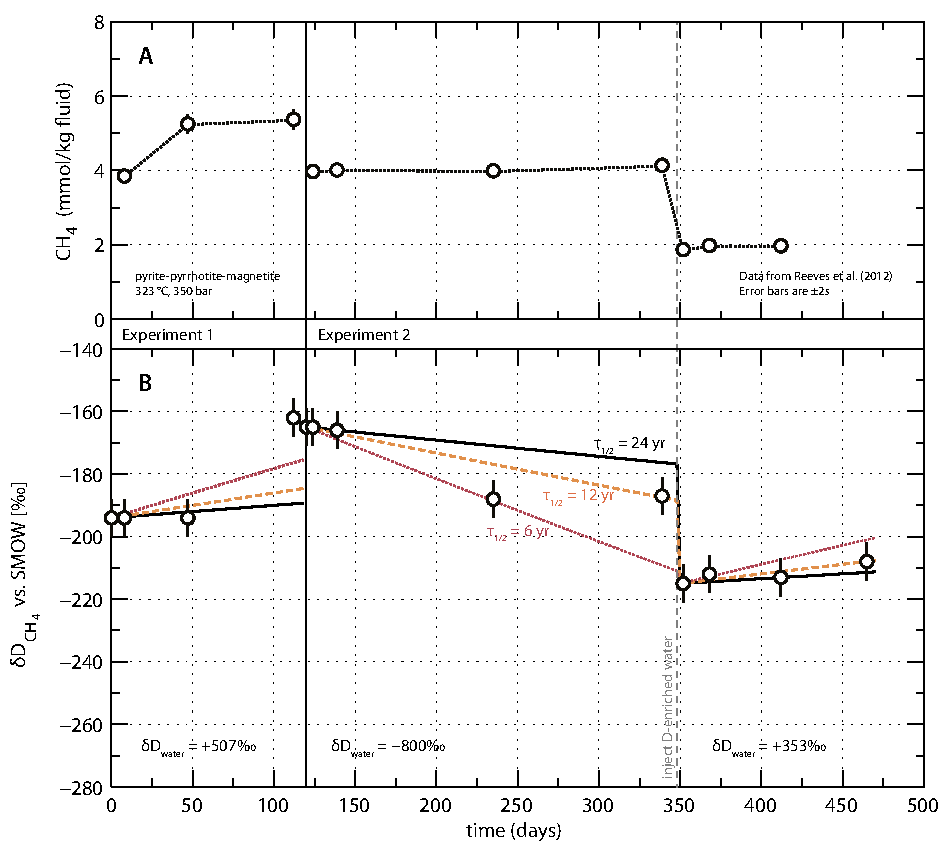
\includegraphics[width=0.95\linewidth]{figures/Fig3.S2}
	\caption[Rates of hydrogen exchange between CH\textsubscript{4}(\emph{aq}) and
	H\textsubscript{2}O(\emph{l}) from data of \textcite{Reeves++_2012_GCA} ]{%
		Experimental constraints on hydrogen
		exchange between CH\textsubscript{4}(\emph{aq}) and
		H\textsubscript{2}O(\emph{l}) from two experiments conducted by \textcite{Reeves++_2012_GCA} in a flexible cell hydrothermal apparatus at 323~°C and
		350~bar. Concentrations of CH\textsubscript{4} (\textbf{A}) remain
		indistinguishable within analytical error (±5\%, 2\emph{s}) in
		Experiment~2, but not in Experiment~1, perhaps due to calibration or operator error as noted by those authors. Measured
		pH was \textasciitilde{}4.2, and concentrations of H\textsubscript{2}
		and $\big\sum\!$H\textsubscript{2}S were 0.26--0.7 mmol/kg fluid and
		\textasciitilde{}11~mmol/kg fluid, respectively, consistent with
		predictions for a Fe--S--O--H fluid buffered by PPM at experimental
		conditions \parencite{Reeves++_2012_GCA}. Panel (\textbf{B}) shows measurements
		of D/H of CH\textsubscript{4} compared against modeled kinetics for D/H
		exchange with varying half-exchange time ($\tau_{1/2} = \ln(2)/k$). The modeled kinetics assume that CH\textsubscript{4}
		concentration is constant, the rate of isotopic exchange is first order
		in CH\textsubscript{4}, and the equilibrium D/H fractionation factor
		{[}$\varepsilon = $ (D/H)\textsubscript{methane}/(D/H)\textsubscript{water} -- 1{]} is
		$-$130‰ (see \autoref{fig:3:5}). We take $\tau_{1/2}$ = 24~yr (black curve)
		as a best-guess estimate of the rate of true isotopic exchange; this
		value is shown in \autoref{fig:3:4}.
	}
	\label{fig:3:S2}
\end{figure*}




